 \documentclass[a4paper,12pt, oneside]{book}

%  Русский язык
\usepackage{cmap}					% Улучшенный поиск русских слов
\usepackage[T2A]{fontenc}			% кодировка
\usepackage[utf8]{inputenc}			% кодировка исходного текста
\usepackage[english,russian]{babel}	% локализация и переносы
\usepackage{pscyr}					% нормальные шрифты

% Колонтитулы
\usepackage{fancybox,fancyhdr}
\usepackage{lastpage}
\fancyhf{}
\fancypagestyle{all}
{
	\fancyhead{}
	\fancyhead[C]{\vspace{-1mm}Контрольная работа 12 Вариант Попов Юрий СКБ-171}
	\fancyfoot{}
	\fancyfoot[C]{\hfill  \thepage  \hfill}
}

% Картинки и графики
\usepackage{wrapfig}
\usepackage{pgfplots}
\pgfplotsset{compat=1.9}
\graphicspath{{fotos/}}


% Ссылки
\usepackage{xcolor}
\usepackage{color,colortbl} % раскраска таблиц
\usepackage[unicode, pdftex]{hyperref}
\definecolor{linkcolor}{HTML}{000000} 	% цвет ссылок
\definecolor{urlcolor}{HTML}{8B000F}	% цвет гиперссылок
\hypersetup{urlcolor=urlcolor, linkcolor=linkcolor, colorlinks=true}

% Размеры
\setlength{\paperwidth}{210mm}
\setlength{\paperheight}{297mm}
\setlength{\textheight}{225mm} 			% высота без колонтитулов
\setlength{\textwidth}{170mm}			% ширина текста
\oddsidemargin=0pt
\setlength{\headheight}{2mm}			% высота колонтитула
\setlength{\headsep}{5mm} 	% от блока текста до верхнего колонтитула
\setlength{\footskip}{10mm}  % от блока текста до нижнего колонтитула

% Математика
\usepackage{amsmath,amsfonts,amssymb,amsthm,mathtools,mathtext} 
\usepackage{latexsym,array,epsfig,wasysym}
\usepackage[all]{xy}
\let\int\varint
\def\Int{\int\limits}
\def\IInt{\iint\limits}
\def\IIInt{\iiint\limits}
\DeclarePairedDelimiter\floor{\lfloor}{\rfloor}


% Оглавление 
\usepackage{setspace}

\usepackage{tocloft} %регулировка расположения TableOfContent (Оглавления) на странице

%\setcounter{tocdepth}{1} % отменяет вывод в оглавление subsection and subsubsection
%\setcounter{secnumdepth}{1} %отменяет номерацию секций в тексте и оглавлении.
\usepackage{tocloft} %регулировка расположения TableOfContent (Оглавления) на странице

\renewcommand{\cfttoctitlefont}{\hspace{0.38\textwidth} \bfseries\MakeUppercase} %уменьшаем размер шрифта и ровняем по центру

% % Межстрочные отступы в Оглавлении:
\setlength{\cftbeforetoctitleskip}{5mm} %отступ Оглавления от верхнего поля страницы.
\setlength{\cftbeforechapskip}{14mm} %отступ между главами
\setlength{\cftbeforesecskip}{5mm} %отступ между секциями \section{title}

% % Отступы от левого поля:
\setlength{\cftchapindent}{1mm} %отступ между левым полем и \chapter{}
\setlength{\cftsecindent}{13mm} %отступ между левым полем и \section{title}

% % Отточия в Оглавлении
\renewcommand\cftchapdotsep{\cftdot} %добавляет отточия после \chapter{title}
%\renewcommand{\cftchapleader}{\cftdotfill{\cftchapdotsep}} %делает отточия после \chapter{title} тонкими, (по умолчанию жирные).
\renewcommand\cftsecdotsep{\cftdot} %делает отточия после \section{title} частыми.

% % Интервалы между абзацами, главами и так далее:
\usepackage{titlesec}

\titleformat{\chapter}[display]
{\filcenter}
{\MakeUppercase{\chaptertitlename} \thechapter}
{2pt}
{\bfseries}{}

\titleformat{\section}
{\normalsize\bfseries}
{\thesection}
{1em}{}

\titleformat{\subsection}
{\normalsize\bfseries}
{\thesubsection}
{1em}{}

% Настройка вертикальных и горизонтальных отступов
\titlespacing*{\chapter}{10pt}{-5pt}{8pt}
\titlespacing*{\section}{\parindent}{*4}{*4}
\titlespacing*{\subsection}{\parindent}{*4}{*4}


\begin{document} % начало документа	
	\pagestyle{plain}
	
	\begin{titlepage}	
		\begin{center}
			{\Huge \textbf{Математическая статистика}}
			\vspace{30mm}
			
			{\Huge Домашняя работа № 3 \\}
			\vspace{30mm}
			
			{\huge Оценки}
			\vspace{30mm}
			
			{\Large Попов Юрий, СКБ-172}
		\end{center}
	\end{titlepage}
	
	
	
\begin{spacing}{0.99}          
	\tableofcontents %Оглавление             
\end{spacing}

\newpage
\begin{center}
	{\Huge{\bf{Предисловие}}}
\end{center}



%-------------------------------------Предисловие

Все графики, которые в дальнейшем будут вставлены в эту работу, были сконструированы с помощью различных библиотек, основные которые - это matplotlib  и numpy в Jupyter Notebook\\

К работе приложены 2 основных файла: "Geom\_Dz\_3.ipynb" и "Expon\_Dz\_3.ipynb" , в которых указаны расчеты  соотвественно геометрического и  экспоненциального распределения\\

Подробности работа с данными находятся в двух других юпитерских файлах: "Database\_Geom\_3.ipynb" и "Database\_Expon\_3\_New.ipynb", в которых находятся расчеты для геометрически и экспоненциально, распределенных данных\\

Все фотографии, использованные в работе лежат в папке {\it fotos}\\

Когда я начинал третье домашнее задание, обновленного файла с домашней работы еще не было( или я не знал о его существовании), поэтому номер 3.2 сделан из старого файла\\


Большая часть определений, которые представлены в этой работы взять с лекций нашего курса. 
\vspace{5mm}

Также некоторые определения взяты из источника   Г.И. Ивченко, Ю.И. Медведев \\
"Ведение в математическую статистику"

%-------------------------------------Предисловие

\setcounter{secnumdepth}{-1} % убираем нумерацию 



\large\textit{\chapter{Задание 3.1 Нахождение выборочного среднего и выборочной дисперсии}}
\vspace{5mm}


\vspace{5mm}
\large{\textbf{Выборочные моменты}}
\vspace{5mm}

Наиболее важными характеристиками случайной величины $\xi$ являются ее моменты $\alpha_k = E\xi^k$, а также центральные моменты $\mu_k = E(\xi - \alpha_1)^k$( когда они существуют). Их статическими аналогами, вычисляемыми по соответствующей выборке $X = (X_1, \ldots, X_n)$, являются {\it выборочные моменты} соответственно {\it обычные}
$$
\hat{\alpha}_k = \frac{1}{n} \sum\limits_{i = 1}^n X_i^k
$$ 
и центральные 
$$
\hat{\mu}_k = \frac{1}{n} \sum\limits_{i = 1}^n (X_i - \hat{\alpha}_1)^k
$$

Особенно важны моменты первого и второго порядков.

При $k = 1$ величину $\hat{\alpha}_1$ называют {\it выборочным средним} и обозначают стандартным символом $\bar{X}$:
$$
\bar{X} = \hat{\alpha}_1 = \frac{1}{n} \sum\limits_{i = 1}^n X_i
$$

При $k = 2$ величину $\hat{\mu}_2$ называют {\it выборочной дисперсией} и  также обозначают стандартным символом $S^2 = S^2(X)$:
$$
S^2 = \hat{\mu}_2 = \frac{1}{n} \sum\limits_{i = 1}^n  (X_i - \bar{X})^2
$$


\vspace{5mm}
\phantomsection
\section{\large{3.1.1 Экспоненциальное распределение}}
\vspace{5mm}

Посчитаем теоритические значения выборочного среднего и выборочной дисперсии. Расчеты будут проводится для $ \lambda = 0.8 $.

\textit{Выборочное среднее:}
$$
MX = \dfrac{1}{\lambda} = \dfrac{1}{0.8} = 1,25
$$

$n = 5 $

$\overline{X} = 1,36$

$\Delta = |MX - \overline X | = 0,11$\\

$n = 10 $

$\overline{X} = 1,85$

$\Delta = |MX - \overline X | = 0,6$\\

$n = 100 $

$\overline{X} = 1,21$

$\Delta = |MX - \overline X | = 0,08$\\

$n = 1000 $

$\overline{X} = 1,33$

$\Delta = |MX - \overline X | = 0,04$\\

$n = 10^5 $

$\overline{X} = 1,248$

$\Delta = |MX - \overline X | = 0,002$\\

\textit{Выборочная дисперсия:}

$$
DX = \dfrac{1}{\lambda^2} = \dfrac{1}{0.8^2} = 1,5625
$$

$n = 5 $

$\hat{\sigma^2} = 0,7$

$\Delta = |DX - \hat{\sigma^2}| = 0,8624$\\

$n = 10 $

$\hat{\sigma^2} = 1,035$

$\Delta = |DX - \hat{\sigma^2}| = 0,5275$\\

$n = 100 $

$\hat{\sigma^2} = 1,153$

$\Delta = |DX - \hat{\sigma^2}| = 0,4$\\


$n = 1000 $

$\hat{\sigma^2} = 1,515$

$\Delta = |DX - \hat{\sigma^2}| = 0,0475$\\

$n = 10^5 $

$\hat{\sigma^2} = 1,563$

$\Delta = |DX - \hat{\sigma^2}| = 0,0005$\\

Из приведенных данных прекрасно видно, что при увлечении объема выборки, то есть при увеличении количества рассматриваемых величин, разница между истинными значениями параметров и значениями их параметров стремится к 0.\\


Это еще раз доказало свойство выборочных моментов - \textit{асимптотическое поведение при неограниченном возрастании объема выборки}. \\

На основании неравенства Чебышева следует, что для любого  $\varepsilon > 0\text{ при } n \rightarrow \infty   $ 
$$
P\{|\hat{\alpha_{nk}} - \alpha_k| < \varepsilon\} \rightarrow 1
$$


\vspace{5mm}
\phantomsection
\textbf{\section{\large{3.1.2 Геометрическое распределение}}}
\vspace{5mm}

Посчитаем теоритические значения выборочного среднего и выборочной дисперсии. Расчеты будут проводится для $ p  = 0.2 $.

\textit{Выборочное среднее:}
$$
MX = \dfrac{1}{p} = \dfrac{1}{0.25} = 4
$$

$n = 5 $

$\overline{X} = 1,4$

$\Delta = |MX - \overline X | = 2,6$\\

$n = 10 $

$\overline{X} = 2,8$

$\Delta = |MX - \overline X | = 1,2$\\

$n = 100 $

$\overline{X} = 3,64$

$\Delta = |MX - \overline X | = 0,36$\\

$n = 1000 $

$\overline{X} = 3,893$

$\Delta = |MX - \overline X | = 0,107$\\

$n = 10^5 $

$\overline{X} = 3,979$

$\Delta = |MX - \overline X | = 0,021$\\

\textit{Выборочная дисперсия:}

$$
DX = \dfrac{1}{p^2} = \dfrac{1}{0.25^2} = 16
$$

$n = 5 $

$\hat{\sigma^2} = 5,04$

$\Delta = |DX - \hat{\sigma^2}| = 10.96$\\

$n = 10 $

$\hat{\sigma^2} = 8,29$

$\Delta = |DX - \hat{\sigma^2}| = 7,71$\\


$n = 100 $

$\hat{\sigma^2} = 12,248$

$\Delta = |DX - \hat{\sigma^2}| = 3,752$\\

$n = 1000 $

$\hat{\sigma^2} = 15,297$

$\Delta = |DX - \hat{\sigma^2}| = 0,703$\\

$n = 10^5 $

$\hat{\sigma^2} = 15,989$

$\Delta = |DX - \hat{\sigma^2}| = 0,011$\\

Объяснение такое же (написано выше)





\phantomsection
\large{ \it \chapter{ Задание 3.2 Построение доверительного интервала для выборочного среднего и выборочной дисперсии}}
\vspace{5mm}



\vspace{5mm}
\phantomsection
\textbf{\section{\large{3.2.1 Геометрическое распределение}}}
\vspace{5mm}

Для всех выборок построим доверительные интервалы.

\begin{figure}[h!]
	\begin{center}
		\begin{minipage}[h]{0.47\linewidth}
			\center{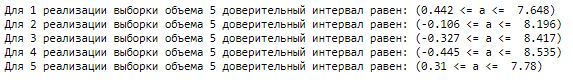
\includegraphics[width=1\linewidth]{fotos/geom_dov_interval_5.jpg}} n = 5 \\
			\vspace{15mm}
		\end{minipage}
		\hfill
		\begin{minipage}[h]{0.47\linewidth}
			\center{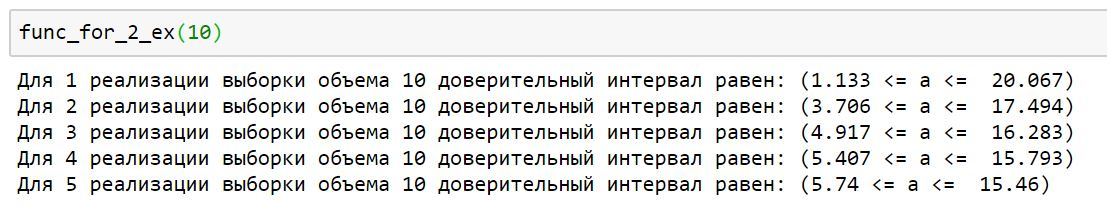
\includegraphics[width=1\linewidth]{fotos/geom_dov_interval_10.jpg}} n = 10 \\
			\vspace{15mm}
		\end{minipage}
		\hfill
		\begin{minipage}[h]{0.47\linewidth}
			\center{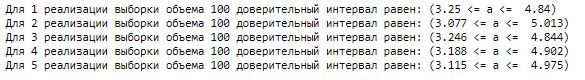
\includegraphics[width=1\linewidth]{fotos/geom_dov_interval_100.jpg}} n = 100 \\
			\vspace{15mm}
		\end{minipage}
		\hfill
		\begin{minipage}[h]{0.47\linewidth}
			\center{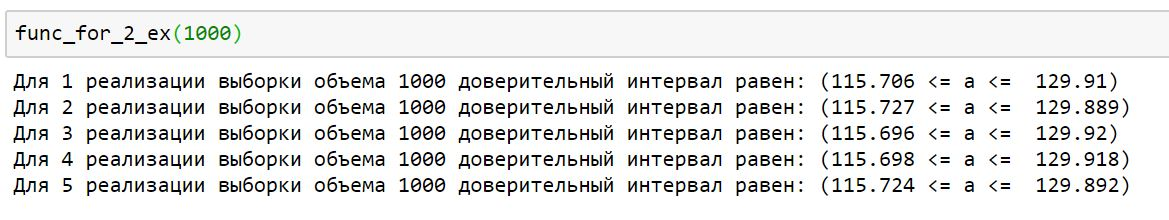
\includegraphics[width=1\linewidth]{fotos/geom_dov_interval_1000.jpg}} n = 1000  \\
			\vspace{15mm}
		\end{minipage}
		\hfill	
		\begin{minipage}[h]{0.47\linewidth}
			\center{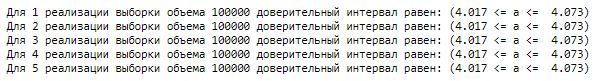
\includegraphics[width=1\linewidth]{fotos/geom_dov_interval_103.jpg}} n = 100000 \\
		\end{minipage}
	\end{center}
\end{figure}




\vspace{5mm}
\phantomsection
\textbf{\section{\large{3.2.2 Экспоненциальное распределение}}}
\vspace{5mm}

Для всех выборок построим доверительные интервалы.

\begin{figure}[h!]
	\begin{center}
		\begin{minipage}[h]{0.47\linewidth}
			\center{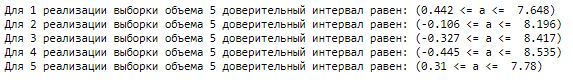
\includegraphics[width=1\linewidth]{fotos/geom_dov_interval_5.jpg}} n = 5 \\
			\vspace{15mm}
		\end{minipage}
		\hfill
		\begin{minipage}[h]{0.47\linewidth}
			\center{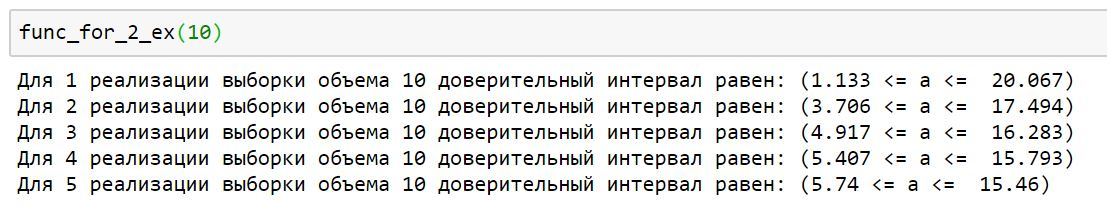
\includegraphics[width=1\linewidth]{fotos/geom_dov_interval_10.jpg}} n = 10 \\
			\vspace{15mm}
		\end{minipage}
		\hfill
		\begin{minipage}[h]{0.47\linewidth}
			\center{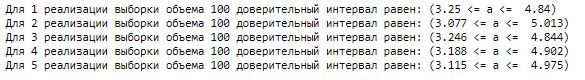
\includegraphics[width=1\linewidth]{fotos/geom_dov_interval_100.jpg}} n = 100 \\
			\vspace{15mm}
		\end{minipage}
		\hfill
		\begin{minipage}[h]{0.47\linewidth}
			\center{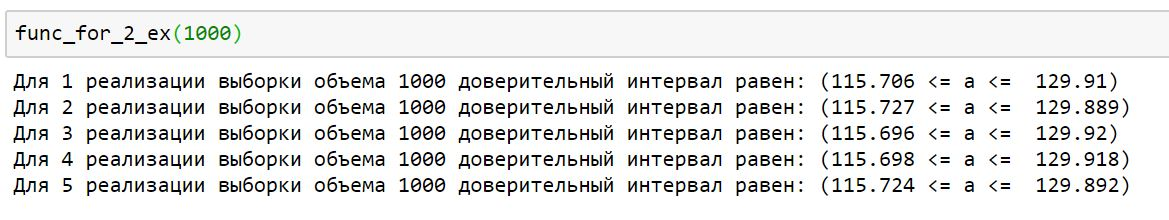
\includegraphics[width=1\linewidth]{fotos/geom_dov_interval_1000.jpg}} n = 1000  \\
			\vspace{15mm}
		\end{minipage}
		\hfill	
		\begin{minipage}[h]{0.47\linewidth}
			\center{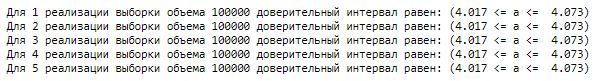
\includegraphics[width=1\linewidth]{fotos/geom_dov_interval_103.jpg}} n = 100000 \\
		\end{minipage}
	\end{center}
\end{figure}



\phantomsection
\vspace{5mm}
\large\textit{\chapter{Задание 3.3 Нахождение параметров распределений событий}}


\textbf{Определение}
	$\mathcal{F} = {F_\theta(x|\theta \in \Theta)}$ называется экспоненциальной, если 
	\[f(x; \theta) = exp(A(\theta)\star B(x) + C(\theta) + D(x)).\]


Для того, чтобы в модели существовала эффективная оценка, необходимо и достаточно, чтобы модель принадлежала экспоненциальному семейству.\\

Вклад выборки для экспоненциальной модели равен:\\

$$
V(X; \theta) = A'(\theta) \sum\limits_{i = 1}^n B(X_i) + n C'(\theta) = n A'(\theta)[\frac{1}{n} \sum\limits_{i=1}^{n} B(X_i) + \dfrac{C'(\theta)}{A'(\theta )}]
$$

Это также можно записать в виде:\\
$$
T(X) - \tau(\theta) = \alpha(\theta) V(x; \theta)
$$

При этом:\\
$$
\tau(\theta) = - \dfrac{C'(\theta)}{A'(\theta )} 
$$

$$
\alpha(\theta) = \dfrac{1}{n A'(\theta)}
$$

$$
T^* = T^*(X) = \frac{1}{n} \sum\limits_{i = 1}^n B(X_i)
$$

По критерию Рао-Крамера заключаем, что статистика $ T^* $ является эффективной оценкой для параметрической функции $ \tau(\theta) $


Оба распределения относятся к экспоненциальному семейству

\vspace{5mm}
\phantomsection
\textbf{\section{\large{3.3.1 Геометрическое распределение}}}
\vspace{5mm}

Найдем оценку для геометрического распределения
$$
P(X=k) = p (1 - p)^{x - 1}, x \in N, p - \text{оцениваемый параметр} 
$$

$$
E[X] = \frac{1}{p}
$$

$$
D(X) = \frac{1-p}{p^2}
$$

Функция правдоподобия:\\

$$
L_\theta = \
$$

$$
\ln(L_\theta) = n \ln(\theta) + n \overline{x}\ln(1 - \theta)
$$

Уравнение правдоподобия имеет вид:\\

$$
\dfrac{\partial \ln(L_\theta)}{\partial \theta} = 0
$$

Продифференцировав, получаем:\\
$$
\dfrac{n}{\theta} + \dfrac{n\overline{x}}{1 - \theta} = 0
$$

$$
\dfrac{\theta \overline{x}}{\theta - 1} = 1
$$

Получаем оценку максимального правдоподобия для $ \theta:  \hat{\theta} = \dfrac{1}{\overline{x}}$\\

Так как оценка получена методом максимального правдоподобия, то она является состоятельной, асимптотически нормальной и эффективной



\vspace{5mm}
\phantomsection
\textbf{\section{\large{3.3.2 Экспоненциальное распределение}}}
\vspace{5mm}

Данное распределение тоже относится к экспоненциальному семейству.\\

Плотность вероятности:\\

$$
f(x, \theta) = e^{-\theta x + \ln\theta}
$$

Найдем все коэффициенты:

$$
A(\theta) = - \theta\\
$$

$$
B(x) = x\\
$$

$$
C(\theta) = \ln\theta\\
$$

$$
D(x) = 0\\
$$ 


$$
T^* = T^*(X) = \frac{1}{n} \sum\limits_{i = 1}^n B(X_i) = \overline{X}
$$

$$
\tau(\theta) = - \dfrac{C'(\theta)}{A'(\theta )}  = -\dfrac{(\ln\theta)'}{(-\theta)'} = \dfrac{1}{\theta}
$$

И наконец получаем оценку параметра $ \theta $:\\
$$
\hat{\theta} = \dfrac{n}{\overline{X}} = \dfrac{n}{\sum\limits_{i = 1}^n X_i}
$$

\textbf{Проверим несмещенность:}
$$
M\hat{\Theta} = M \dfrac{n}{\sum_{i= 1}^{n} X_i} = n M \dfrac{1}{\sum_{i = 1}^{n} X_i}
$$

Воспользуемся связью между распределениями, и так как $ X_i $ распределена экспоненциально, то сумма $ X_i $ будет иметь распределение Эрланга с параметрами $ n  $ и $ \theta $. Получаем:
$$
M\hat{\theta} = \dfrac{n \theta}{n - 1}
$$

Итог: оценка является смещенной.

Если оценка смещенная, то она не является эффективной. Построим несмещенную оценку $ \theta $:
$$
\hat{\theta} = \dfrac{n - 1}{n} \dfrac{n}{\sum_{i = 1}^{n} X_i} = \dfrac{n-1}{\sum_{i = 1}^{n} X_i}
$$

$$
M\tilde{\theta} = \theta 
$$

\textbf{Проверим состоятельность:}
$$
D \tilde{\theta} = M\tilde{\theta ^2}  - (M \tilde{\theta})^2 
$$
$$
M\tilde{\theta ^2} =  (n - 1)^2 M(\dfrac{1}{\sum_{i = 1}^{n}X_i})^2 = (n-1)^2 \dfrac{Г(n - 2)}{Г(n)} \theta^2 = \dfrac{n - 1}{n -2 }\theta^2
$$
$$
D \tilde{\theta} = M\tilde{\theta ^2}  - (M \tilde{\theta})^2  = \dfrac{n - 1}{n -2}\theta^2 - \theta^2 = \dfrac{\theta^2}{(n - 2)}
$$

Итог: так как $ D\tilde{\theta} \rightarrow 0 \text{ при }  \infty$, то оценка будет состоятельной.

Так как распределение принадлежит экспоненциальному семейству, то достаточная статистика для параметра является полной\\

\textbf{Проверим на достаточную статистику}

Докажем, что  $ \overline(X) $ является достаточной статистикой для $ \theta $

$$
L(x , \theta) = \ln (\prod\limits_{i = 1}^n \theta e^{-\theta x_i}) = \theta^n \ln(\prod\limits_{i = 1}^n \theta e^{-\theta n \overline{X}}) = n \ln\theta - \theta n \overline{X} = n(\ln \theta - \theta \overline{X} )
$$

Соотвественно, так как выполняется критерий факторизации, то $ T(X) = \overline{X} $ является достаточной статистикой и значит полной статистикой.\\

\textbf{Проверим на оптимальность}

По теореме Рао-Блэкулла-Колмагорова - оптимальная оценка, если существует является функцией от достаточной статистики. Если статистика полная, то можно сделать и обратное утверждение. Функция от полной и достаточной статистики является оптимальной.

Оценка $ T(\dfrac{n -1 }{\sum_{i =1}^{n } X_i}) = \dfrac{1 - 1/n}{\overline{X}} $  является функцией от достаточной полной статистики, а значит по теореме является оптимальной.



\phantomsection
\vspace{5mm}
\large\textit{\chapter{Задание 3.4 Работа с данными}}

\vspace{5mm}
\phantomsection
\textbf{\section{\large{3.4.1 Геометрическое распределение}}}
\vspace{5mm}

В перовой домашней работе в качестве нетипичной интерпретации геометрического распределения была выбрана модель, в которой рассматривается ДНК, то есть последовательность 4 видов нуклеотидов, и, например,  перед исследователями стоит задача изучить  частоту встречаемости какого-то определенного вида. Соответственно, без особых трудностей мной была найдена база данных, показывающая весь геном после применения метода дробовика.\cite{rt3} Метод дробовика - метод, используемый для секвенирования  длинных участков ДНК.  Суть метода состоит в получении случайной массированной выборки клонированных фрагментов ДНК данного организма, на основе которых может быть восстановлена исходная последовательность ДНК. \\


Итак, моя выборка состоит из последовательности нуклеотидов 'A', 'C', 'G','T'. Анализируя эту выборку, я считал расстояние между двумя соседними нуклеотидами 'T'. Я начал двигаться по ДНК, установив при этом счетчик на значение 1. Соответственно, при каждой встрече нужного нуклеотида, значение счетчика заносилось в отдельный массив, затем счетчик устанавливался на значение 1 и движение продолжалось. \\

В результате анализа, я построил функцию вероятности моей выборки. Синим цветом - теоретически построена функция вероятности с подобранным коэффициентом.\\

\begin{figure}[h!]
	\begin{center}
		\begin{minipage}[h]{0.47\linewidth}
			\center{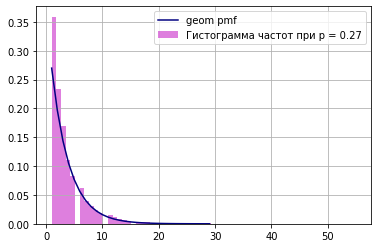
\includegraphics[scale = 1]{fotos/database/Geom/hist.png}}  \\
			\vspace{15mm}
		\end{minipage}
	\end{center}
\end{figure}

Затем были посчитаны выборочное среднее и выборочная дисперсия. И согласно, полученной мною ранее оптимальной оценки, получена оценка параметра. Они приблизительно оказались равны!!!

\begin{figure}[h!]
	\begin{center}
		\begin{minipage}[h]{0.47\linewidth}
			\center{
\includegraphics[width=1\linewidth]{fotos/database/Geom/1.jpg}}\\
			\vspace{15mm}
		\end{minipage}
		\hfill	
		\begin{minipage}[h]{0.47\linewidth}
			\center{\includegraphics[width=1\linewidth]{fotos/database/Geom/2.jpg}} \\
		\end{minipage}
		\end{center}
\end{figure}



\newpage
\phantomsection
\textbf{\section{\large{3.4.2 Экспоненциальное распределение}}}
\vspace{5mm}

В первой домашней работе в качетсве нетипичной интерпретации для экспоненциального распределения была выбрана теория надежности. Эта интерпретация позволяет исследовать срок службы прибора или механизма, и в нужный момент принять соответствующие меры по ремонту или замене деталей. \\

Я нашел базу данных, касающуюся безработицы. В этой базе данных главным фактором была приведена продолжить безработицы, то есть количество дней, которое она продолжалась\\

Почему, я считаю, что данная интерпретация соответствует экспоненциальному распределению? Работа, или другой похожий способ заработка, определяет доход человека, и соотвественно, его возможности.  Если человек, по какой либо причине потеряет работу, то ему будет нечем себя кормить и не на что будет существовать. Но так, как, возможно, что у него(нее) есть накопления, то он сможет спокойно жить без работы, но так как иной прибыли денег нет, то в какой-то момент накопления будут заканчиваться, и жизнь заставит искать работу. Так что со временем, человек перестанет быть безработным\\

Этот процесс очень схож с жизнью приборов. Чем дольше прибор находится в эксплотации, тем выше вероятность, что он выйдет из строя, а в случае человека - найдет работу.\\ 

Для этих данных я проделал тоже самое, что и для предыдущих. \\

Получил вот такие результаты: 


\begin{figure}[h!]
	\begin{center}
		\begin{minipage}[h]{0.47\linewidth}
			\center{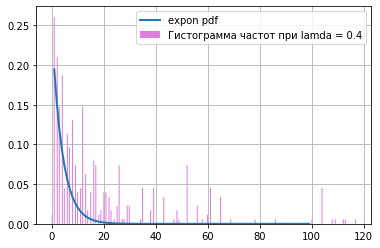
\includegraphics[scale = 0.8]{fotos/database/Expon/hist.png}}  \\
			\vspace{15mm}
		\end{minipage}
	\end{center}
\end{figure}

Они приблизительно оказались равны!!!

\begin{figure}[h!]
	\begin{center}
		\begin{minipage}[h]{0.47\linewidth}
			\center{
\includegraphics[width=1\linewidth]{fotos/database/Expon/1.jpg}}\\
			\vspace{15mm}
		\end{minipage}
		\hfill	
		\begin{minipage}[h]{0.47\linewidth}
			\center{\includegraphics[width=1\linewidth]{fotos/database/Expon/2.jpg}} \\
		\end{minipage}
	\end{center}
\end{figure}



\chapter{ Регулярность }

Статистическая модель называется \textit{регулярной} (по Рао-Крамеру), если выполнены следующие условия, которые в дальнейшем будем называть условиями регулярности:


\begin{enumerate}
	\item $L(\bar{x}; \theta) > 0$ и дифференцируема по $\theta, \; \forall \theta \in \Theta$ ( $\Theta$ --- параметрическое множество).
	\item Случайная величина $V(x; \theta)$, называемая функцией вклада выборки и определенная равенством
	\[V(x; \theta) = \frac{\partial \ln (L(\bar{x}; \theta))}{\partial \theta} = \sum \limits_{i = 1}^{\infty} \frac{\partial \ln(f_i(x_i;\theta))}{\partial \theta},\] имеет ограниченную дисперсию:
	\[0 < E V^2(X; \theta) < \infty. \] При этом значение $\cfrac{\partial \ln(f_i(x_i;\theta))}{\partial \theta}$  будем называть вкладом выборки.
	\item $\forall \theta \in \Theta$ $\forall$ статистики $T(X)$ верно равенство:
	\[
	\frac{\partial}{\partial \theta} \int T(x) L(\bar{x}; \theta) dx = \int T(x) \frac{\partial L(\bar{x}; \theta)}{\partial \theta} dx.
	\]
\end{enumerate}


Оба распределения являются регулярными моделями. 

Так как перед нами степенной ряд, то мы можем спокойно менять знаки интегрирования и дифференцирования под знаком суммы.

\begin{thebibliography}{99}
	\bibitem{rt1} 
	\bibitem{rt2} \href{https://vincentarelbundock.github.io/Rdatasets/datasets.html}{Ссылка на базу данных для экспоненциального распределения,Unemployment,  Unemployment Duration}
	\bibitem{rt3}  \href{https://www.ncbi.nlm.nih.gov/nuccore/NC_024460.2?report=fasta&from=10460803&to=10470316}{Ссылка на базу данных для геометрического распределения, NCBI - National Center of Biotechnology Information}
	\bibitem{rt4}  // \href{http://www.ams.jhu.edu/~dan/550.435/notes/COURSENOTES435.pdf}{ссылка3}
	\bibitem{rt5}  // \href{http://www.obzh.ru/nad/4-3.html}{ссылка4}
\end{thebibliography}

\end{document}